\documentclass[a4paper, 12pt]{report}

\usepackage[dvipsnames]{xcolor}

%%%%%%%%%%%%%%%%
% Set Variables %
%%%%%%%%%%%%%%%%

\def\useItalian{0}  % 1 = Italian, 0 = English

\def\courseName{Mathematical Logic for Computer Science}

\def\coursePrerequisites{TODO}

\def\book{TODO}

% \def\authorName{Simone Bianco}
% \def\email{bianco.simone@outlook.it}
% \def\github{https://github.com/Exyss/university-notes}
% \def\linkedin{https://www.linkedin.com/in/simone-bianco}

\def\authorName{Alessio Bandiera}
\def\email{alessio.bandiera02@gmail.com}
\def\github{https://github.com/aflaag-notes}
\def\linkedin{https://www.linkedin.com/in/alessio-bandiera-a53767223}

%%%%%%%%%%%%
% Packages %
%%%%%%%%%%%%

\usepackage{../../packages/Nyx/nyx-packages}
\usepackage{../../packages/Nyx/nyx-styles}
\usepackage{../../packages/Nyx/nyx-frames}
\usepackage{../../packages/Nyx/nyx-macros}
\usepackage{../../packages/Nyx/nyx-title}
\usepackage{../../packages/Nyx/nyx-intro}

%%%%%%%%%%%%%%
% Title-page %
%%%%%%%%%%%%%%

\logo{../../packages/Nyx/logo.png}

\if\useItalian1
    \institute{\curlyquotes{\hspace{0.25mm}Sapienza} Università di Roma}
    \faculty{Ingegneria dell'Informazione,\\Informatica e Statistica}
    \department{Dipartimento di Informatica}
    \ifdefined\book
        \subtitle{Appunti integrati con il libro \book}
    \fi
    \author{\textit{Autore}\\\authorName}
\else
    \institute{\curlyquotes{\hspace{0.25mm}Sapienza} University of Rome}
    \faculty{Faculty of Information Engineering,\\Informatics and Statistics}
    \department{Department of Computer Science}
    \ifdefined\book
        \subtitle{Lecture notes integrated with the book \book}
    \fi
    \author{\textit{Author}\\\authorName}
\fi


\title{\courseName}
\date{\today}

% \supervisor{Linus \textsc{Torvalds}}
% \context{Well, I was bored\ldots}

\addbibresource{./references.bib}

%%%%%%%%%%%%
% Document %
%%%%%%%%%%%%

\begin{document}
    \maketitle

    % The following style changes are valid only inside this scope 
    {
        \hypersetup{allcolors=black}
        \fancypagestyle{plain}{%
        \fancyhead{}        % clear all header fields
        \fancyfoot{}        % clear all header fields
        \fancyfoot[C]{\thepage}
        \renewcommand{\headrulewidth}{0pt}
        \renewcommand{\footrulewidth}{0pt}}

        \romantableofcontents
    }

    \introduction

    %%%%%%%%%%%%%%%%%%%%%

    \chapter{TODO}

    \section{Introduction}

    placeholder \todo{missing introduction}

    \begin{frameddefn}{Languages and propositions}
        A \tbf{propositional language} is a --- possibly infinite --- set $\mathcal L = \{p_1, \ldots, p_n\}$, where each $p_i$ is called \tbf{propositional variable}. Given a propositional language $\mathcal L$, the set of \tbf{propositions} over $\mathcal L$, denoted with $\textsf{PROP}_{\mathcal L}$ is inductively defined as follows:

        \begin{itemize}
            \item each propositional variable in $\mathcal L$ is a proposition, i.e. $\mathcal L \subseteq \textsf{PROP}_{\mathcal L}$
            \item if $A \in \textsf{PROP}_{\mathcal L}$, then $\lnot A \in \textsf{PROP}_{\mathcal L}$
            \item if $A, B \in \textsf{PROP}_{\mathcal L}$, then $(A \land B), (A \lor B), (A \rightarrow B), (A \leftrightarrow B) \in \textsf{PROP}_{\mathcal L}$
        \end{itemize}
    \end{frameddefn}

    In other words, the set of propositions over a language is the set of \tit{formulas} that can be constructed from the initial variables of $\mathcal L$, by using the Boolean connectives. Note that a propositional language may have an infinite number of propositional variables, even \tit{uncountably infinite}. For instance, the following is a valid propositional language $$\mathcal L := \{p_r \mid r \in \R\}$$ However, since propositions are inductively constructed starting from variables, each proposition of any language $\mathcal L$ will still be defined over a \tit{finite} number of propositional variables of $\mathcal L$.

    Now that we provided a formal definition for languages and propositions, we are ready to discuss \tbf{assignments}.

    \begin{frameddefn}{Assignment}
        Given a propositional language $\mathcal L$, an \tbf{assignment} $\alpha$ is a function $\func{\alpha}{\mathcal L}{\{0, 1\}}$ that assigns either 0 or 1 to all of $\mathcal L$'s propositional variable.
    \end{frameddefn}

    This definition can be inductively extended to \tbf{propositions} themselves: if $A$ and $B$ are two propositions, let $\func{\widehat \alpha}{\textsf{PROP}_{\mathcal L}}{\{0, 1\}}$ be a function such that

    $$A \in \mathcal L \implies \widehat \alpha (A) = \alpha(A)$$
    
    $$\widehat \alpha(\lnot A) = \soe{ll}{1 & \widehat \alpha(A) = 0 \\ 0 & \mathrm{otherwise}}$$

    $$\widehat \alpha(A \land B) = \soe{ll}{1 & \widehat \alpha(A) = \widehat \alpha(B) = 1 \\ 0 & \mathrm{otherwise}}$$

    $$\widehat \alpha(A \lor B) = \soe{ll}{1 & \widehat \alpha(A) = 1 \lor \widehat \alpha(B) = 1 \\ 0 & \mathrm{otherwise}}$$

    $$\widehat \alpha(A \rightarrow B) = \soe{ll}{0 & \widehat \alpha(A) = 1 \land \widehat \alpha(B) = 0 \\ 0 & \mathrm{otherwise}}$$

    $$\widehat \alpha(A \leftrightarrow B) = \soe{ll}{1 & \widehat \alpha(A) = \widehat \alpha (B) \\ 0 & \mathrm{otherwise}}$$

    Since it can be proven that the extension $\widehat \alpha$ of $\alpha$ is unique, we will refer to $\widehat \alpha$ as $\alpha$ directly. Two propositions $A$ and $B$ are said to be \tbf{equivalent} --- written as $A \equiv B$ --- if and only if $\forall \alpha \quad \alpha(A) = \alpha(B)$.

    \begin{frameddefn}{Satisfiability}
        A proposition $A$ is said to be \tbf{satisfiable} if there exists an assignment $\alpha$ of its propositional variables such that $\alpha(A) = 1$. If there is no assignment that satisfies $A$, $A$ is said to be \tbf{unsatisfiable}, and if $A$ is satisfied for any assignment $\alpha$, then $A$ is said to be a \tbf{tautology}.

        We will denote with \SAT, \UNSAT and \TAUT respectively the sets of all satisfiable propositions, all unsatisfiable propositions and all tautologies.
    \end{frameddefn}

    Using symbols, we have that

    \begin{itemize}
        \item $A \in \SAT \iff \exists \alpha \quad \alpha (A) = 1$
        \item $A \in \UNSAT \iff \nexists \alpha \quad \alpha (A) = 1 \iff \forall \alpha \quad \alpha (A) = 0$
        \item $A \in \TAUT \iff \forall \alpha \quad \alpha(A) = 1 \iff \nexists \alpha \quad \alpha (A) = 0$
    \end{itemize}
    
    The concept of satisfiability is strictly related to the concept of \tbf{logical consequence}, which is defined as follows.

    \begin{frameddefn}{Logical consequence}
        Given the propositions $A_1, \ldots, A_n, A$, we say that $A$ is a \tbf{logical consequence} of $A_1, \ldots, A_n$ if whenever $A_1, \ldots, A_n$ are true, $A$ is also true. We will indicate this concept as follows: $$A_1, \ldots, A_n \models A$$
    \end{frameddefn}

    From its definition, the concept of logical consequence can be alternatively be expressed in terms of \tit{unsatisfiability} and \tit{tautology}.

    \begin{framedthm}{}
        Given the formulas $A_1, \ldots, A_n, A$, the following statements are equivalent:

        \begin{itemize}
            \item $A_1, \ldots, A_n \models A$
            \item $(A_1 \land \ldots \land A_n \rightarrow A) \in \TAUT$
            \item $(A_1 \land \ldots \land A_n \land A) \in \UNSAT$
        \end{itemize}
    \end{framedthm}

    \subsection{Theories}

    \begin{frameddefn}{Theory}
        Given a language $\mathcal L$, a \tbf{theory} $T$ over $\mathcal L$ is a --- finite or infinite --- set of propositions defined on $\mathcal L$, i.e. $T \subseteq \textsf{PROP}_{\mathcal L}$.
    \end{frameddefn}

    As a natural extension of the \tit{satisfiability} property previously discussed, a theory $T$ will be said to be \tbf{satisfiable} --- written as $T \in \SAT$ if and only if $$\exists \alpha \quad \alpha(T) = 1$$ which is equivalent of saying that $$\exists \alpha \quad \forall F \in T \quad \alpha (F) = 1$$ note that the assignment $\alpha$ must be the same for all the propositions $F$ of $T$.

    Additionally, for infinite theories we can define another property.

    \begin{frameddefn}{Finite satisfiability}
        An infinite theory $T$ is said to be \tbf{finitely satisfiable} if and only if $$\forall T' \subset T \ \mathrm{finite} \quad T' \in \SAT$$ We will denote with $\FINSAT$ the set of all finitely satisfiable theories.
    \end{frameddefn}
    
    However, the following theorem will prove that \tit{satisfiability} and \tit{finite satisfiability} are actually \tbf{equivalent}.

    \begin{framedthm}{Compactness theorem (1st version)}
        Given an infinite theory $T$, it holds that $$T \in \SAT \iff T \in \FINSAT$$
    \end{framedthm}

    \begin{proof}
        In this proof we will assume that the propositions of the infinite theory $T$ are \tit{countably infinite}, however in its general form this theorem can be proved even without this assumption.

        Since the direct implication of this statement is trivially true by definition, we just need to prove the converse implication.

        \claim{
            Given a theory $T \in \FINSAT$, and a proposition $A$, it must hold that $T \cup \{A\} \in \FINSAT$ or $T \cup \{\lnot A \} \in \FINSAT$.
        }{
            By way of contradiction, assume that $T \cup \{A\}, T \cup \{\lnot A\} \notin \FINSAT$.

            By definition of finite satisfiability, if $T \cup \{A\} \notin \FINSAT$, then there must exist a \tit{finite} sub-theory $T_0 \subset T \cup \{A\}$ such that $T_0 \in \UNSAT$. Note that $T \in \FINSAT$, therefore if $T \cup \{A\} \notin \FINSAT$ then it must be that $A \in T_0$. Let $\widehat{T_0}$ be the theory such that $T_0 := \widehat{T_0} \cup \{A\}$; then $$T_0 := \widehat{T_0} \cup \{A\} \in \UNSAT \iff \forall \alpha  \quad \alpha(T_0) = 0$$ which implies that $$\forall \alpha \quad \alpha(\widehat{T_0}) = 1 \implies \alpha(A) = 0$$

            Analogously, we can apply the same reasoning for $T \cup \{\lnot A\}$, and we get that there must exist a \tit{finite} sub-theory $T_1 \subset T \cup \{\lnot A\}$ such that $T_1 := \widehat{T_1} \cup \{\lnot A\} \in \UNSAT$, which implies that $$\forall \alpha \quad \alpha (\widehat{T_1}) = 1 \implies \alpha(\lnot A) = 0$$

            Lastly, since $\widehat{T_0} \cup \widehat{T_1} \subset T \in \FINSAT$, by finite satisfiability of $T$ there must exist an assignment $\alpha$ such that $\alpha(\widehat{T_0} \cup \widehat{T_1}) = 1$, and therefore $\alpha(\widehat{T_0}) = \alpha(\widehat{T_1}) = 1$. However, for the previous observations this implies that $\alpha(A) = \alpha(\lnot A) = 0 \ \lightning$.
        }

        Since we are assuming that the propositions of $T$ are \tit{countably infinite}, and the number of variables in any proposition is finite by definition, we can fix an enumeration $p_1, p_2, p_3, \ldots$ on the --- possibly infinite --- propositional variables of $T$. Given this enumeration, define the following \tit{chain} of sub-theories:
        
        \begin{itemize}
            \item $T_0 := T$
            \item $T_{i + 1} := \soe{ll}{T_i \cup \{p_i \} & T_i \cup \{p_i\} \in \FINSAT \\ T_i \cup \{\lnot p_i\} & T_i \cup \{\lnot p_i\} \in \FINSAT}$
        \end{itemize}

        and note that, by definition, clearly $$T =: T_0 \subseteq T_1 \subseteq T_2 \subseteq \ldots$$ Moreover, let $$T^* := \bigcup_{i \in \N}{T_i}$$ and note that since $\forall i \quad T_i \in \FINSAT$ by definition, then it must be that $T^* \in \FINSAT$ as well, as $T^*$ is a chain defined \tit{only} by inclusions of \FINSAT theories.

        Now, consider the following assignment: $$\funcmap{\alpha^*}{\{p_1, p_2, \ldots\}}{\{0,1\}}{p_i}{\soe{ll}{1 & p_i \in T^* \\ 0 & \lnot p_i \in T^*}}$$ Note that this assignment is well defined, because by construction of $T^*$ only one between $p_i \in T^*$ and $\lnot p_i \in T^*$ can hold.

        \claim{
            $\alpha^*(T) = 1$.
        }{
            Let $A \in T$, and let $p_{i_1}, \ldots, p_{i_k}$ the be the propositional variables that appear in $A$. Then, for each $j \in [k]$ let $$p_{i_j}^* := \soe{ll}{p_{i_j} & p_{i_j} \in T^* \\ \lnot p_{i_j} & \lnot p_{i_j} \in T^*}$$ and consider the set $\cbk{A, p_{i_1}^*, \ldots, p_{i_k}^*}$. Clearly, this is a finite subset of $T^*$ --- by definition of the various $T_0, T_1, T_2, \ldots$ that define $T^*$ --- hence $T^* \in \FINSAT$ implies that there must exist an assignment $\beta_A$ that satisfies this set, i.e. $$\beta_A(A) = \beta_A \rbk{p_{i_1}^*} = \ldots = \beta_A \rbk{p_{i_k}^*} = 1$$ Note that, for each $j \in [k]$, it holds that $$p_{i_j} \in T^* \implies p_{i_j}^* = p_{i_j} \land \alpha^*\rbk{p_{i_j}} = 1$$ and $1 = \beta_A (p_{i_j}^*) = \beta_A \rbk{p_{i_j}}$; analogously, it holds that $$\lnot p_{i_j} \in T^* \implies p_{i_j}^*= \lnot p_{i_j} \land \alpha^ *\rbk{p_{i_j}} = 0$$ and $1 = \beta_A (p_{i_j}^*) = \beta_A \rbk{\lnot p_{i_j}} = \lnot \beta_A \rbk{p_{i_j}} \implies \beta_A \rbk{p_{i_j}} = 0$. This proves that $\alpha^* \equiv \beta_A$ for all of $A$'s variables, therefore it must also be true that $\alpha^*(A) = \beta_A(A)$.

            Hence, this shows that for any proposition $A \in T$ there is an assignment $\beta_A$, which satisfies $A$, that sets $A$'s variables as $\alpha^*$ does. Therefore, since this will be true for any of the $T$'s propositions, $\alpha^*$ satisfies $T$.
        }

        This claim proves that there exists an assignment $\alpha ^*$ that satisfies $T$, hence $T \in \SAT$, concluding the proof.
    \end{proof}

    The statement of this theorem is equivalent to the following one.

    \begin{framedthm}{Compactness theorem (2nd version)}
        Given an infinite theory $T$, and a proposition $A$, it holds that $$T \models A \iff \exists T' \subset T \ \mathrm{finite} \quad T' \models A$$
    \end{framedthm}
    
    \proofiff{
        We will prove the equivalence of the two formulations by assuming that the first version implies the second version of the theorem, and vice versa. First, notice that if there exist a $T' \subset T$ finite sub-theory of $T$ such that $T' \models A$ for some proposition $A$, then it is trivially true that $T \models A$ by definition of logical consequence. Hence, we just need to prove the direct implication of the second version of the theorem, assuming that the first version it true.

        By way of contradiction, assume that $T \models A$ and for each $T' \subset T$ finite sub-theory of $T$, $T' \not\models A$. By definition of logical consequence, this implies that $$\forall T' \subset T \ \mathrm{finite} \quad \exists \alpha \quad \alpha(T') = 1 \land \alpha(A) = 0$$ or, equivalently, $\alpha(\lnot A) = 1$. This implies that $$\forall T' \subset T \ \mathrm{finite} \quad \exists \alpha \quad \alpha(T' \cup \{\lnot A\}) = 1$$ which means that any finite subset of $T \cup \{\lnot A\}$ is \SAT (recall that $T' \subset T$). Hence, by definition $T \cup \{\lnot A\} \in \FINSAT$, and since we are assuming the first version of the theorem, we have that $$T \cup \{\lnot A \} \in \FINSAT \iff T \cup \{\lnot A\} \in \SAT$$ which implies that $T \not\models A$ by definition of logical consequence.
    }{
        Consider a theory $T$ and a proposition $A$; by the second version of the theorem we know that $T \models A$ if and only if there is a finite sub-theory $T' \subset T$ such that $T' \models A$. Now, suppose that $T \in \UNSAT$; therefore, by definition we have that $T \models 0$, which implies that $$T \models 0 \iff \exists T' \subset' T \ \mathrm{finite} \quad T' \models 0$$ but again, $T' \models 0$ means that $T' \in \UNSAT$. Hence, we proved that $$T \in \UNSAT \iff \exists T' \subset T \ \mathrm{finite} \quad T' \in \UNSAT \iff T \notin \FINSAT$$ which is the contrapositive of the first version of the theorem.
    }
   
    The compactness theorem can be proven to be equivalent to a special case of \href{https://en.wikipedia.org/wiki/K%C5%91nig%27s_lemma}{Kőnig's lemma} \cite{koenig}, which states the following.

    \begin{framedlem}{Kőnig's lemma (special case)}
        Every infinite tree contains either a vertex of infinite degree, or an infinite path.
    \end{framedlem}

    \newpage

    \begin{framedprob}{}
    \end{framedprob}

    \begin{framedprob}{}
    \end{framedprob}

    \begin{framedprob}{}
    \end{framedprob}

    \newpage

    \begin{framedprob}{}
        Let $\mathcal L = \{E(x, y)\}$ be the language of graphs.

        \begin{enumerate}
            \item For each fixed $n \in \N$, write a sentence $C_n$ such that for any graph $\mathcal G$, $\mathcal G \models C_n$ if and only if $\mathcal G$ contains a cycle of length $n$
            \item Prove using Compactness that the property of being \tit{a cycle} is not expressible by a theory in $\mathcal L$ over the class of graphs.
        \end{enumerate}
    \end{framedprob}

    \solution{
        Let $\mathcal L = \{E(x, y)\}$ be the language of graphs.

        \begin{enumerate}
            \item The property \curlyquotes{$\mathcal G$ contains a cycle of length $n$} can be written as follows $$C_n := \exists x_1, \ldots, \exists x_n \quad \rbk{\bigwedge_{1 \le i, j \le n}{\lnot(x_i = x_j)}} \land \rbk{\bigwedge_{1 \le i \le n - 1}{E(x_i, x_{i + 1})} \land E(x_n, x_1)}$$ In fact, the first conjunction implies that $x_1, \ldots, x_n$ are \tit{distinct}, and the second conjunction describes the \tit{cycle} itself (of length $n$).
            \item Consider the property $P_n$ := \curlyquotes{$\mathcal G$ is \tit{a cycle} of length $n$}. This property can be expressed by \tit{extending} $C_n$: in particular, $P(\mathcal G)$ holds if $\mathcal G$ is a cycle and has $n$ vertices, therefore we need to add to $C_n$ the following
                \begin{equation*}
                    \begin{split}
                        V_n &:= \rbk{\forall y \rbk{\bigvee_{1 \le j \le p}{(y = x_j)}}} \\
                        E^{C_n}_n &:= \displaystyle \bigwedge_{1 \le i \le n}{\bigwedge_{\substack{1 \le j \le n : \\ j \neq n + 1}}{\lnot E(x_i, x_j)}} \\
                        C'_n &:= \exists x_1, \ldots \exists x_n \quad C_n \land V_n \land E^{C_n}_n$
                    \end{split}
                \end{equation*}
                where we have that

                \begin{itemize}
                    \item $V_n$ forces that $\mathcal G$ has \tit{exactly} $n$ vertices
                    \item $E^{C_n}_n$ forces that the only edges present in $\mathcal G$ are the ones that describe the cycle graph of $n$ vertices
                    \item $C'_n$ describes our property $P_n$
                \end{itemize}

                Now, consider the property $P$ := \curlyquotes{$\mathcal G$ is \tit{a cycle}}, and in particular $\lnot P$ := \curlyquotes{$\mathcal G$ is not \tit{a cycle}}. We observe that we can build the following infinte theory $$T^{\lnot P} := \{\lnot C_n' \mid n \in \N \}$$ for which it is easy to see that $$\mathcal G \models \lnot P \iff \lnot P(\mathcal G) \ \mathrm{holds}$$ meaning that $\lnot P$ is expressible through $T^{\lnot P}$.

                \claim{
                    $T^{\lnot P} \in \FINSAT$.
                }{
                    Fix $T_0 \underset{fin}{\subseteq} T^{\lnot P}$. We observe that $T_0 := \{\lnot C_{i_1}', \ldots, \lnot C_{i_k}'\}$ for some $i_1, \ldots, i_k \in \N$. Now, if we consider $\displaystyle i^* := \max_{j \in [k]}{i_j}$, then the cycle graph that has $i^* + 1$ vertices is clearly a structure that satisfies $T_0$.
                }

                \claim{
                    $P$ is not expressible by a theory in $\mathcal L$ over the class of graphs.
                }{
                    By way of contradiction, suppose that $P$ is expressible, i.e. there is a theory $T^P$ for which $P$ can be expressed. Then, consider the theory $T := T^P \cup T^{\lnot P}$. By the previous claim, we have that $T \in \FINSAT$, and by Compactness this is true if and only if $T \in \SAT$. However, this is a contradiction, because a graph cannot be and not be a cycle at the same time.
                }
        \end{enumerate}
    }

    \newpage
    
    \chapter{placeholder}
    
    \newpage

    \begin{framedprob}{}
        Consider the following two structures $\mathcal G_1$ and $\mathcal G_2$ for the languages of graphs:

        \begin{figure}[H]
            \centering

            \begin{tabular}{ccc}
                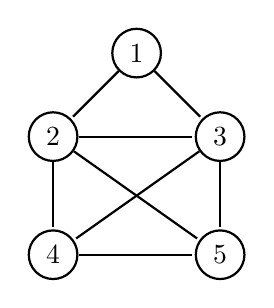
\begin{tikzpicture}[-,>=stealth,shorten >=1pt,auto,node distance=1.5cm, thick,main node/.style={scale=0.9,circle,draw,font=\sffamily\normalsize}]

                    \node[circle, draw]  (1) []{1};
                    \node[circle, draw]  (2) [below left of = 1]{2};
                    \node[circle, draw]  (3) [below right of = 1]{3};
                    \node[circle, draw]  (4) [below of = 2]{4};
                    \node[circle, draw]  (5) [below of = 3]{5};

                    \draw[-] (1) to (2);
                    \draw[-] (1) to (3);
                    \draw[-] (2) to (3);
                    \draw[-] (2) to (4);
                    \draw[-] (2) to (5);
                    \draw[-] (3) to (4);
                    \draw[-] (3) to (5);
                    \draw[-] (4) to (5);

                    ;
                \end{tikzpicture}

                &\qquad\qquad&

                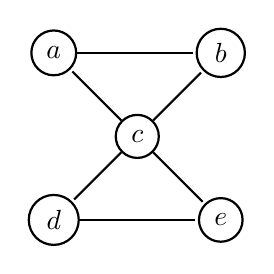
\begin{tikzpicture}[-,>=stealth,shorten >=1pt,auto,node distance=1.5cm, thick,main node/.style={scale=0.9,circle,draw,font=\sffamily\normalsize}]

                    \node[circle, draw]  (1) []{$c$};
                    \node[circle, draw]  (2) [above left of = 1]{$a$};
                    \node[circle, draw]  (3) [above right of = 1]{$b$};
                    \node[circle, draw]  (4) [below left of = 1]{$d$};
                    \node[circle, draw]  (5) [below right of = 1]{$e$};

                    \draw[-] (1) to (2);
                    \draw[-] (1) to (3);
                    \draw[-] (2) to (3);
                    \draw[-] (1) to (4);
                    \draw[-] (1) to (5);
                    \draw[-] (4) to (5);

                    ;
                \end{tikzpicture}
            \end{tabular}
            % \caption{On the left: a simple graph. On the right: a simple digraph.}
        \end{figure}

        Write at least two sentences distinguishing the two structures. Discuss the EF-game played on these structures: for what $k$ can the Duplicator win the $k$-rounds game? For what $k$ can the Spoiler win?
    \end{framedprob}

    \solution{
        Two properties that can distinguish these two structures are the following:

        \begin{enumerate}
            \item \curlyquotes{$\mathcal G$ contains a cycle of length 4}, which is represented by the following sentence $$\exists x_1 \exists x_2 \exists x_3 \exists x_4 \quad \rbk{\bigwedge_{1 \le i, j \le 4}{\lnot(x_i = x_j)}} \land \rbk{\bigwedge_{1 \le i \le 3}{E(x_i, x_{i + 1})} \land E(x_4, x_1)}$$
            \item \curlyquotes{$\mathcal G$ contains a vertex of degree 3}, which is represented by the following sentence \centeredeq{0.9}{$\displaystyle \exists x_1 \exists x_2 \exists x_3 \exists x_4 \quad \rbk{\bigwedge_{1 \le i, j \le 4}{\lnot(x_i = x_j)}} \land \rbk{\bigwedge_{2 \le i \le 4}{E(x_1, x_i)}} \land \rbk{\forall y \rbk{\lnot E(x, y) \lor \bigvee_{2 \le j \le 4}{(y = x_j)}}}$}
            \item descrizione di G1 (e il contrario non va bene)
            \item esistenza di C5
            \item esistenza di K4
            \item esistono due vertici per cui per ogni terzo faccio K3
        \end{enumerate}

        These sentences \tit{may} seem to suggest that the two structures are 3-equivalent, meaning that there is no sentence of rank 3 that can distinguish $\mathcal G_1$ and $\mathcal G_2$. For now, let's focus on proving that they are \tit{at least} 2-equivalent.

        \claim{
            The Duplicator wins $G_2(\mathcal G_1, \mathcal G_2)$.
        }{
            Let $s_i$ and $d_i$ be the $i$-th nodes chosen by the Spoiler and the Duplicator, respectively. Then, we can define the following strategy for the Duplicator:

            \begin{itemize}
                \item if $s_1 \in \{1, 4, 5\}$, then the Duplicator chooses $d_1 \in \{a, b, c, d\}$, otherwise if $s_1 \in \{2, 3\}$ then $d_1 = c$
                \item if $s_1 \in \{a, b, c, d\}$, then the Duplicator chooses $d_1 \in \{1, 4, 5\}$, otherwise if $s_1 = c$ then $d_1 \in \{2, 3\}$
            \end{itemize}

            Then, no matter the choice of $s_2$, the Duplicator can always answer with a node $d_2$ that preserves the partial isomorphism:

            \begin{itemize}
                \item if $s_2 \sim s_1$, it is guaranteed that there is a vertex $d_2$ in the other structure such that $d_2 \sim d_1$ because $\delta_{\mathcal G_1} = \delta_{\mathcal G_2} = 2$ --- and the same argument applies if $s_2 \sim d_1$ for finding a vertex $d_2 \sim s_1$
                \item if $s_2 \nsim s_1$, the strategy that we provided for the Duplicator guarantees that there exists at least one vertex $d_2$ in the other structure such that $d_2 \nsim d_1$ --- and the same argument applies if $s_2 \nsim d_1$ for finding a vertex $d_2 \nsim s_1$
            \end{itemize}

            Thus, the Duplicator has a strategy to always win at least 2 rounds, therefore the Duplicator wins $G_2(\mathcal G_1, \mathcal G_2)$.
        }

        Now, is it true that we are 3-equivalent? Unfortunately, this is not true, as we are going to show in the following claim.

        \claim{
            The Spoiler wins $G_3(\mathcal G_1, G_2)$.
        }{
            The following is a strategy that guarantees the Spoiler to win in 3 rounds:

            \begin{itemize}
                \item let $s_1 \in \{4, 5\}$
                \item by the previous claim, we know that the strategy for the Duplicator to win at least 2 rounds is to choose $d_1 \in \{a, b, d, e\}$, thus we may assume that $d_1 \neq c$
                \item now, let $s_2 = 1$
                \item to preserve the partial isomorphism, we observe that
                    \begin{itemize}
                        \item if $d_1 \in \{a, b\}$, then $d_2 \in \{d, e\}$
                        \item if $d_1 \in \{d, e\}$, then $d_2 \in \{a, b\}$
                    \end{itemize}
                \item now, it suffices for the Spoiler to choose $s_3$ in $\mathcal G_2$ such that $s_3 \sim d_2$ and $s_3 \neq c$: by construction of $\mathcal G_2$, we see that $s_3 \nsim d_1$, but all the vertices in $\{2, 3, 5\}$ are adjacent to $s_1$, which would violate the partial isomorphism
            \end{itemize}
        }

        In fact, we can actually find a property that distinguishes $\mathcal G_1$ and $\mathcal G_2$, which can be written through a sentence of 3 quantifiers: \curlyquotes{there are two vertices $x_1$ and $x_2$ of $\mathcal G$ such that for each third vertex $x_3$ there is a $K_3$ as subgraph of $\mathcal G$ such that $V(K_3) = \{x_1, x_2, x_3\}$} $$\exists x_1 \exists x_2 \forall x_3 \quad \rbk{\bigwedge_{1 \le i, j \le 3}{\lnot (x_i = x_j)}} \land E(x_1, x_2) \land E(x_2, x_3) \land E(x_3, x_1)$$ Let $x_1$, $x_2$ and $x_3$ be the three choosen vertices --- and we may assume that $x_1 \sim x_2$ otherwise the sentence is trivially not satisfied; then, we observe that

        \begin{itemize}
            \item in $\mathcal G_1$ if $x_1, x_2 \in \{2, 3\}$, then for any other vertex $x_3 \in \{1, 4, 5\}$ we can always find a $K_3$ having $x_1$, $x_2$ and $x_3$ as nodes
            \item in $\mathcal G_2$ we have two cases
                \begin{itemize}
                    \item if $\{x_1, x_2\} = \{a, b, c\}$, the property is unsatisfied for $x_3 \in \{d, e\}$
                    \item if $\{x_1, x_2\} = \{c, d, e\}$, the property is unsatisfied for $x_3 \in \{a, b\}$
                \end{itemize}
        \end{itemize}

        In conclusion, we have that $\mathcal G_1 \equiv_2 \mathcal G_2$, and that $\mathcal G_1 \not\equiv_3 \mathcal G_2$.
    }

    \printbibliography % UNCOMMENT FOR BIBLIOGRAPHY

\end{document}
